\begin{frame}
\frametitle{Giới thiệu}
\begin{figure}[htbp]
    \centering
    % Ảnh bên trái
    \begin{subfigure}[t]{0.45\textwidth}
        \centering
        
\includegraphics[width=2cm, height=3cm]{Slides/figure/free fall.png}
        \caption{Rơi tự do}
    \end{subfigure}
    \hfill
    % Ảnh bên phải
    \begin{subfigure}[t]{0.45\textwidth}
        \centering
        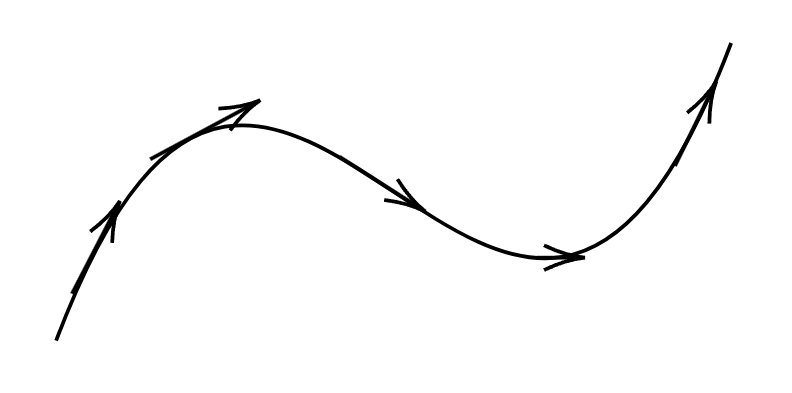
\includegraphics[width=3cm, height=2cm]{Slides/figure/curvature.png}
        \caption{Một đường cong}
    \end{subfigure}
    \caption{Hai thay đổi điển hình-thời gian,và hướng.}
\end{figure}
Giải tích là toán học nghiên cứu sự thay đổi.
\end{frame}
\begin{frame}
\frametitle{Sơ lược lịch sử}
    \begin{figure}[htbp]
    \centering
    % Ảnh bên trái
    \begin{subfigure}[t]{0.45\textwidth}
        \centering
        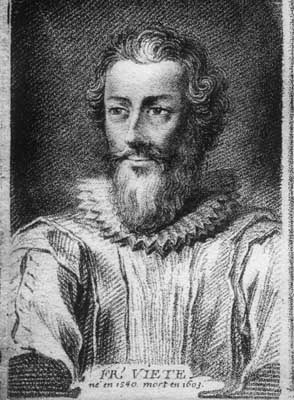
\includegraphics[width=4cm, height=5cm]{Slides/figure/Francois_Viete.jpeg}
        \caption{Francois Viete (1540-1603)}
    \end{subfigure}
    \hfill
    % Ảnh bên phải
    \begin{subfigure}[t]{0.45\textwidth}
        \centering
        \includegraphics[width=4cm, height=5cm]{Slides/figure/Frans_Hals_-_Portret_van_René_Descartes.jpg}
        \caption{René Descartes (1596-1650)}
    \end{subfigure}
    \caption{Sự phát triển của đại số  và hình học giải tích.}
\end{figure}
\end{frame}
\begin{frame}
\frametitle{Sơ lược lịch sử}    
     \begin{figure}[htbp]
    \centering
    % Ảnh bên trái
    \begin{subfigure}[t]{0.45\textwidth}
        \centering
        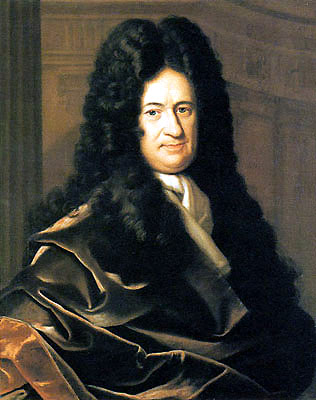
\includegraphics[width=4cm, height=5cm]{Slides/figure/Gottfried_Wilhelm_von_Leibniz.jpg}
        \caption{G.W.Leibniz (1646-1716)}
    \end{subfigure}
    \hfill
    % Ảnh bên phải
    \begin{subfigure}[t]{0.45\textwidth}
        \centering
        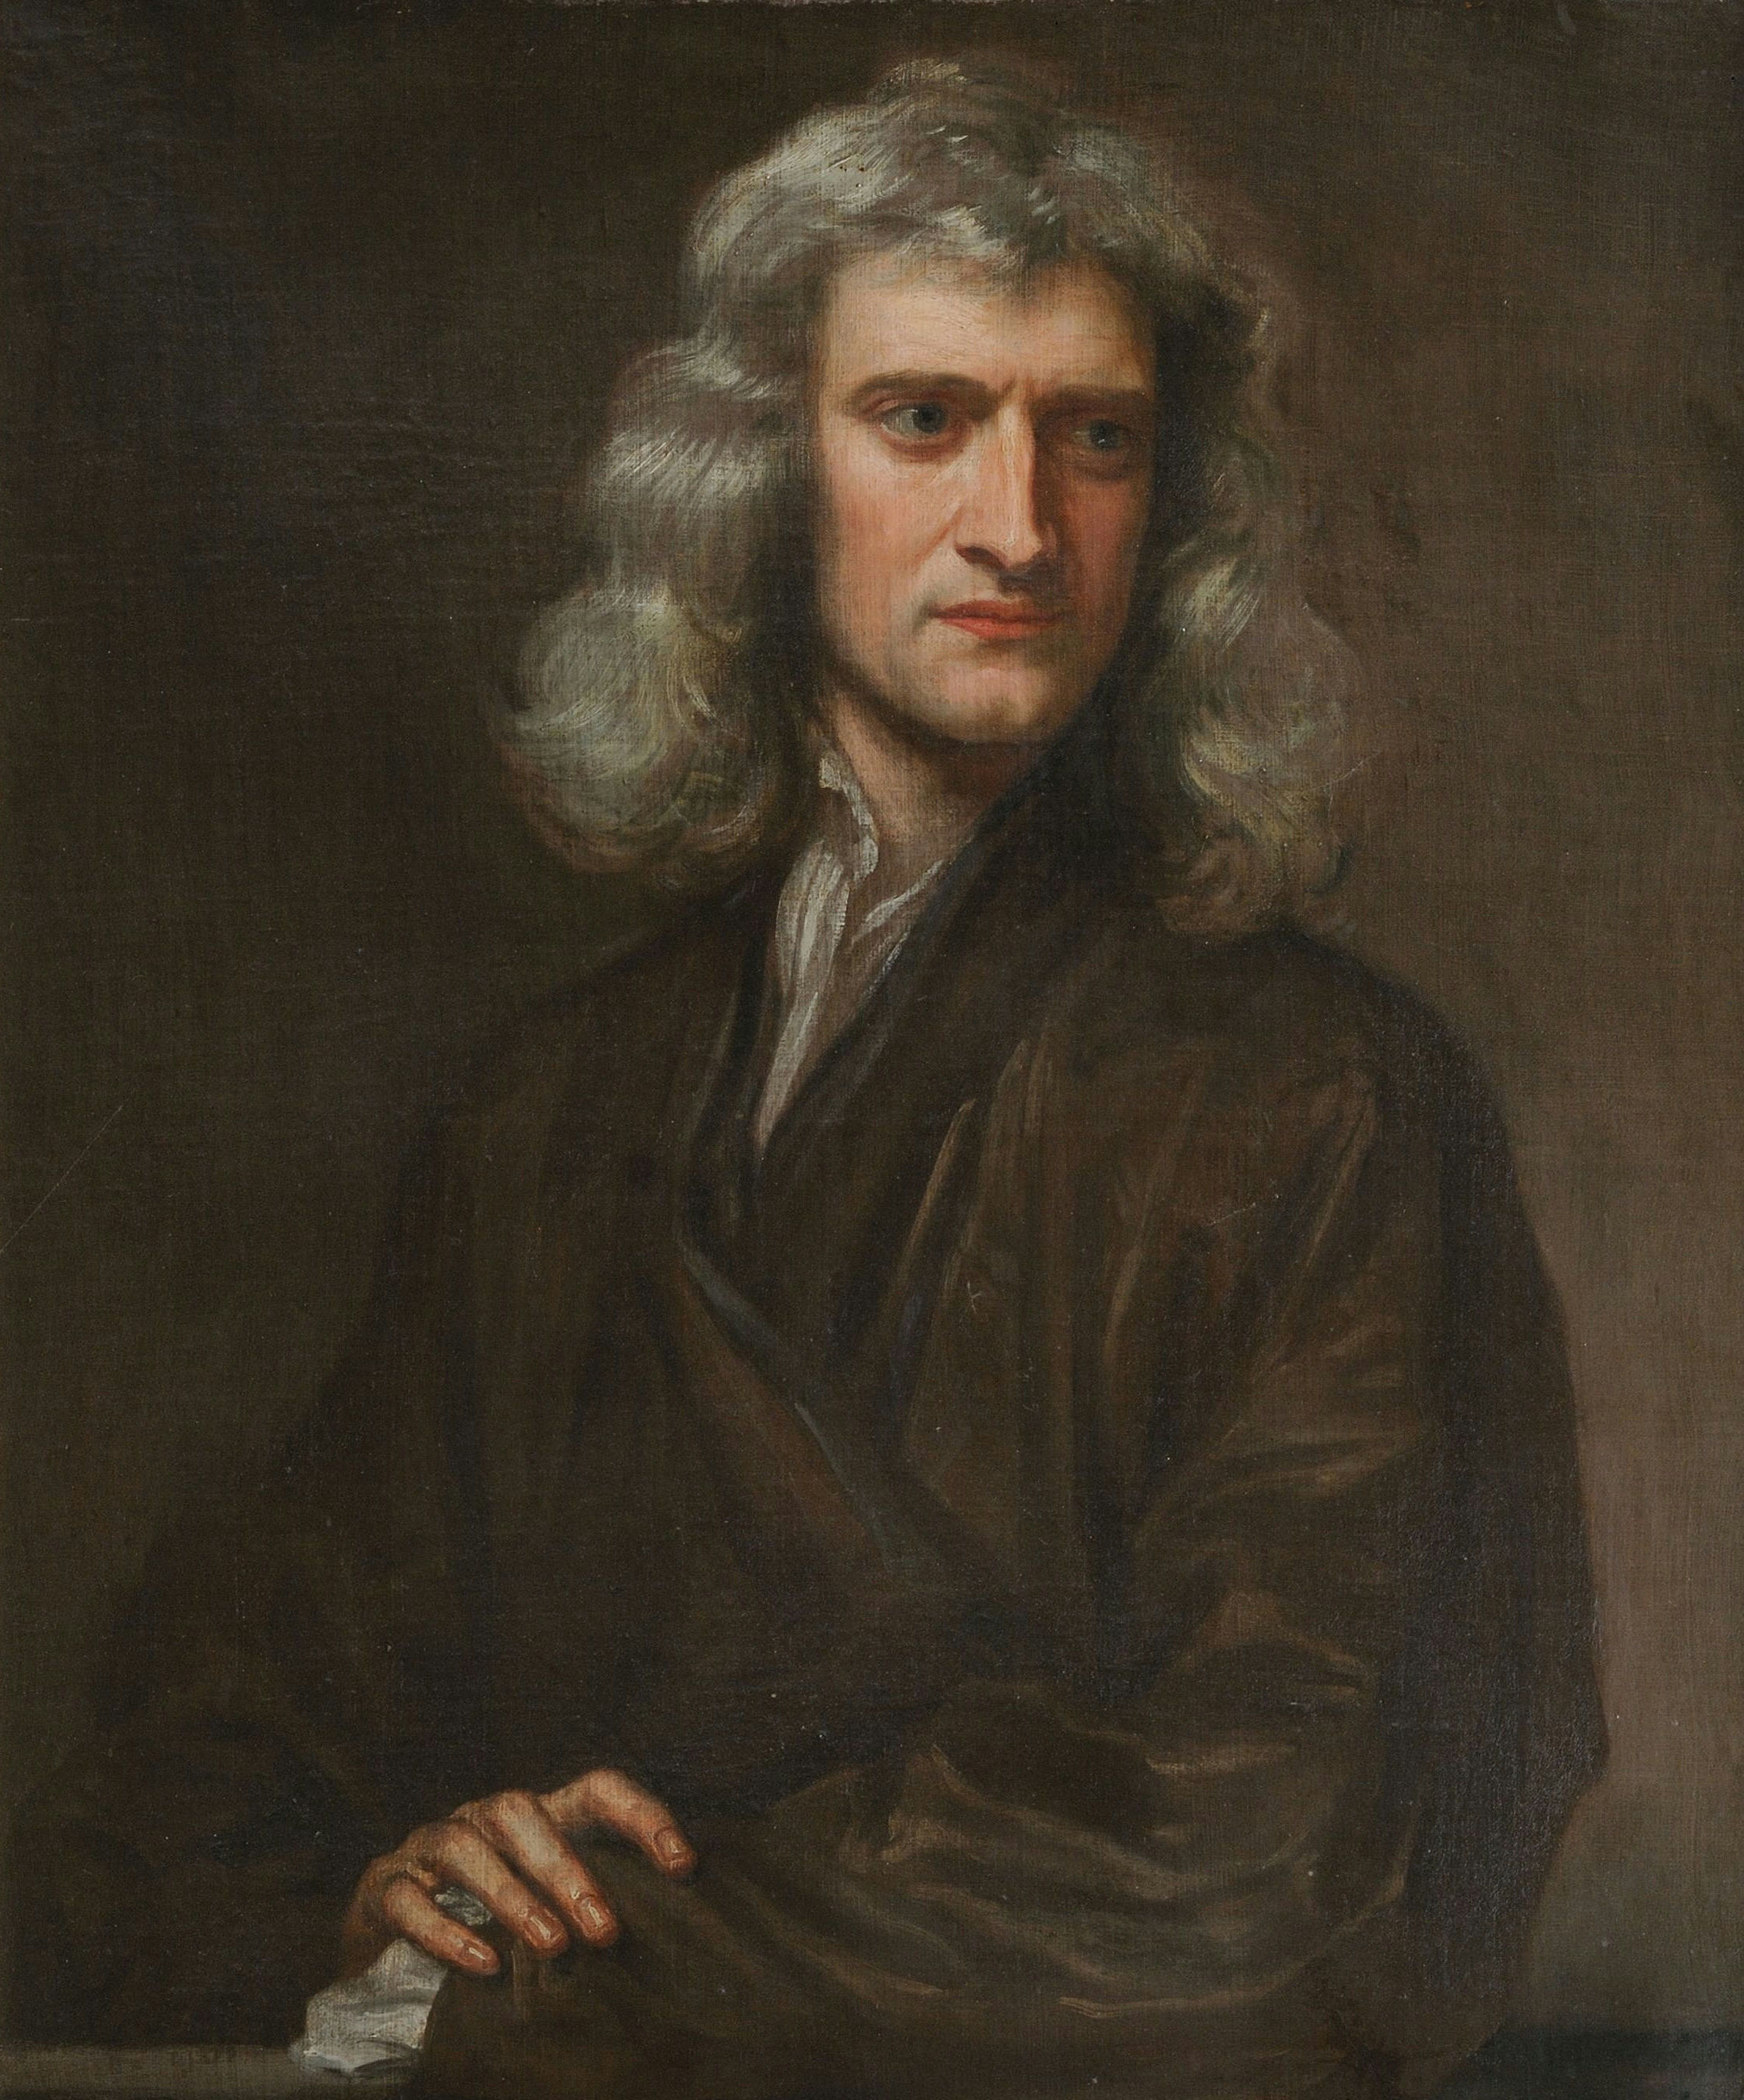
\includegraphics[width=4cm, height=5cm]{Slides/figure/Portrait_of_Sir_Isaac_Newton,_1689.jpg}
        \caption{Isaac Newton (1642-1727)}
    \end{subfigure}
\end{figure}
\end{frame}

\begin{frame}{Hình học giải tích}
    \begin{figure}[htbp]
    \centering
    % Ảnh bên trái
    \begin{subfigure}[t]{0.45\textwidth}
        \centering
        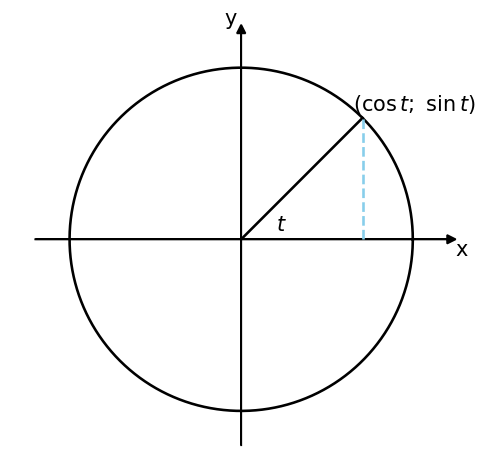
\includegraphics[width=3.5cm, height=3cm]{Slides/figure/duongtronthamso - Copy.png}
    \end{subfigure}
    \hfill
    % Ảnh bên phải
    \begin{subfigure}[t]{0.45\textwidth}
        \centering
        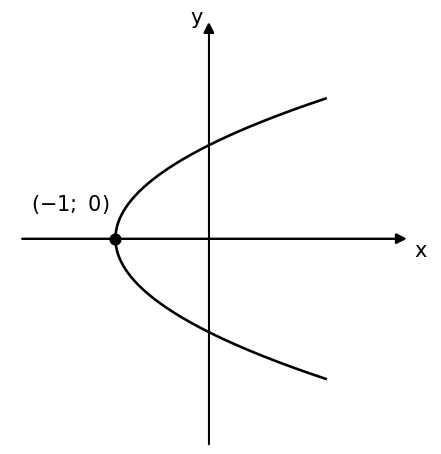
\includegraphics[width=3.5cm, height=3cm]{Slides/figure/parabolngang - Copy.png}
    \end{subfigure}
    \hfill
    \begin{subfigure}[t]{0.45\textwidth}
        \centering
        
\includegraphics[width=3cm, height=3cm]{Slides/figure/cardioid - Copy.png}
    \end{subfigure}
    \hfill
    \begin{subfigure}[t]{0.45\textwidth}
        \centering
        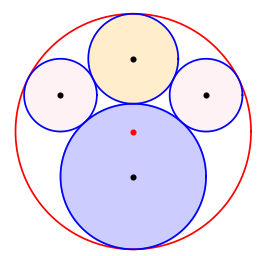
\includegraphics[width=3cm, height=3cm]{Slides/figure/4circle.png}
    \end{subfigure}
\end{figure}
\end{frame}